\chapter{Testing software by setting up a Lab}

    To do own measurements on programm's energy consumption, a new testing Lab will be set up. As far as possible, the criteria of Blue Angel are followed, but due to the range of this project, it is not possible to arrange every point of the needed circumstances.
    In the following chapter the whole measuring process will be described, as well as which tech-stack and software is needed. The main goal is to show the differences of energy consumption between programs.


    \section{Software and Hardware requirements for the lab setup}
    For performing real software test, a few preparatios have to be made. The most important components to reach that are the power meter and two PCs, the first one for Processing the data and the second one for running the scripts with the three usage scenarios (KDE Eco Handbook).
    The following image, created by Lana Lutz (KDE) gives a good overview:

    \begin{figure}[ht]
    \centering
    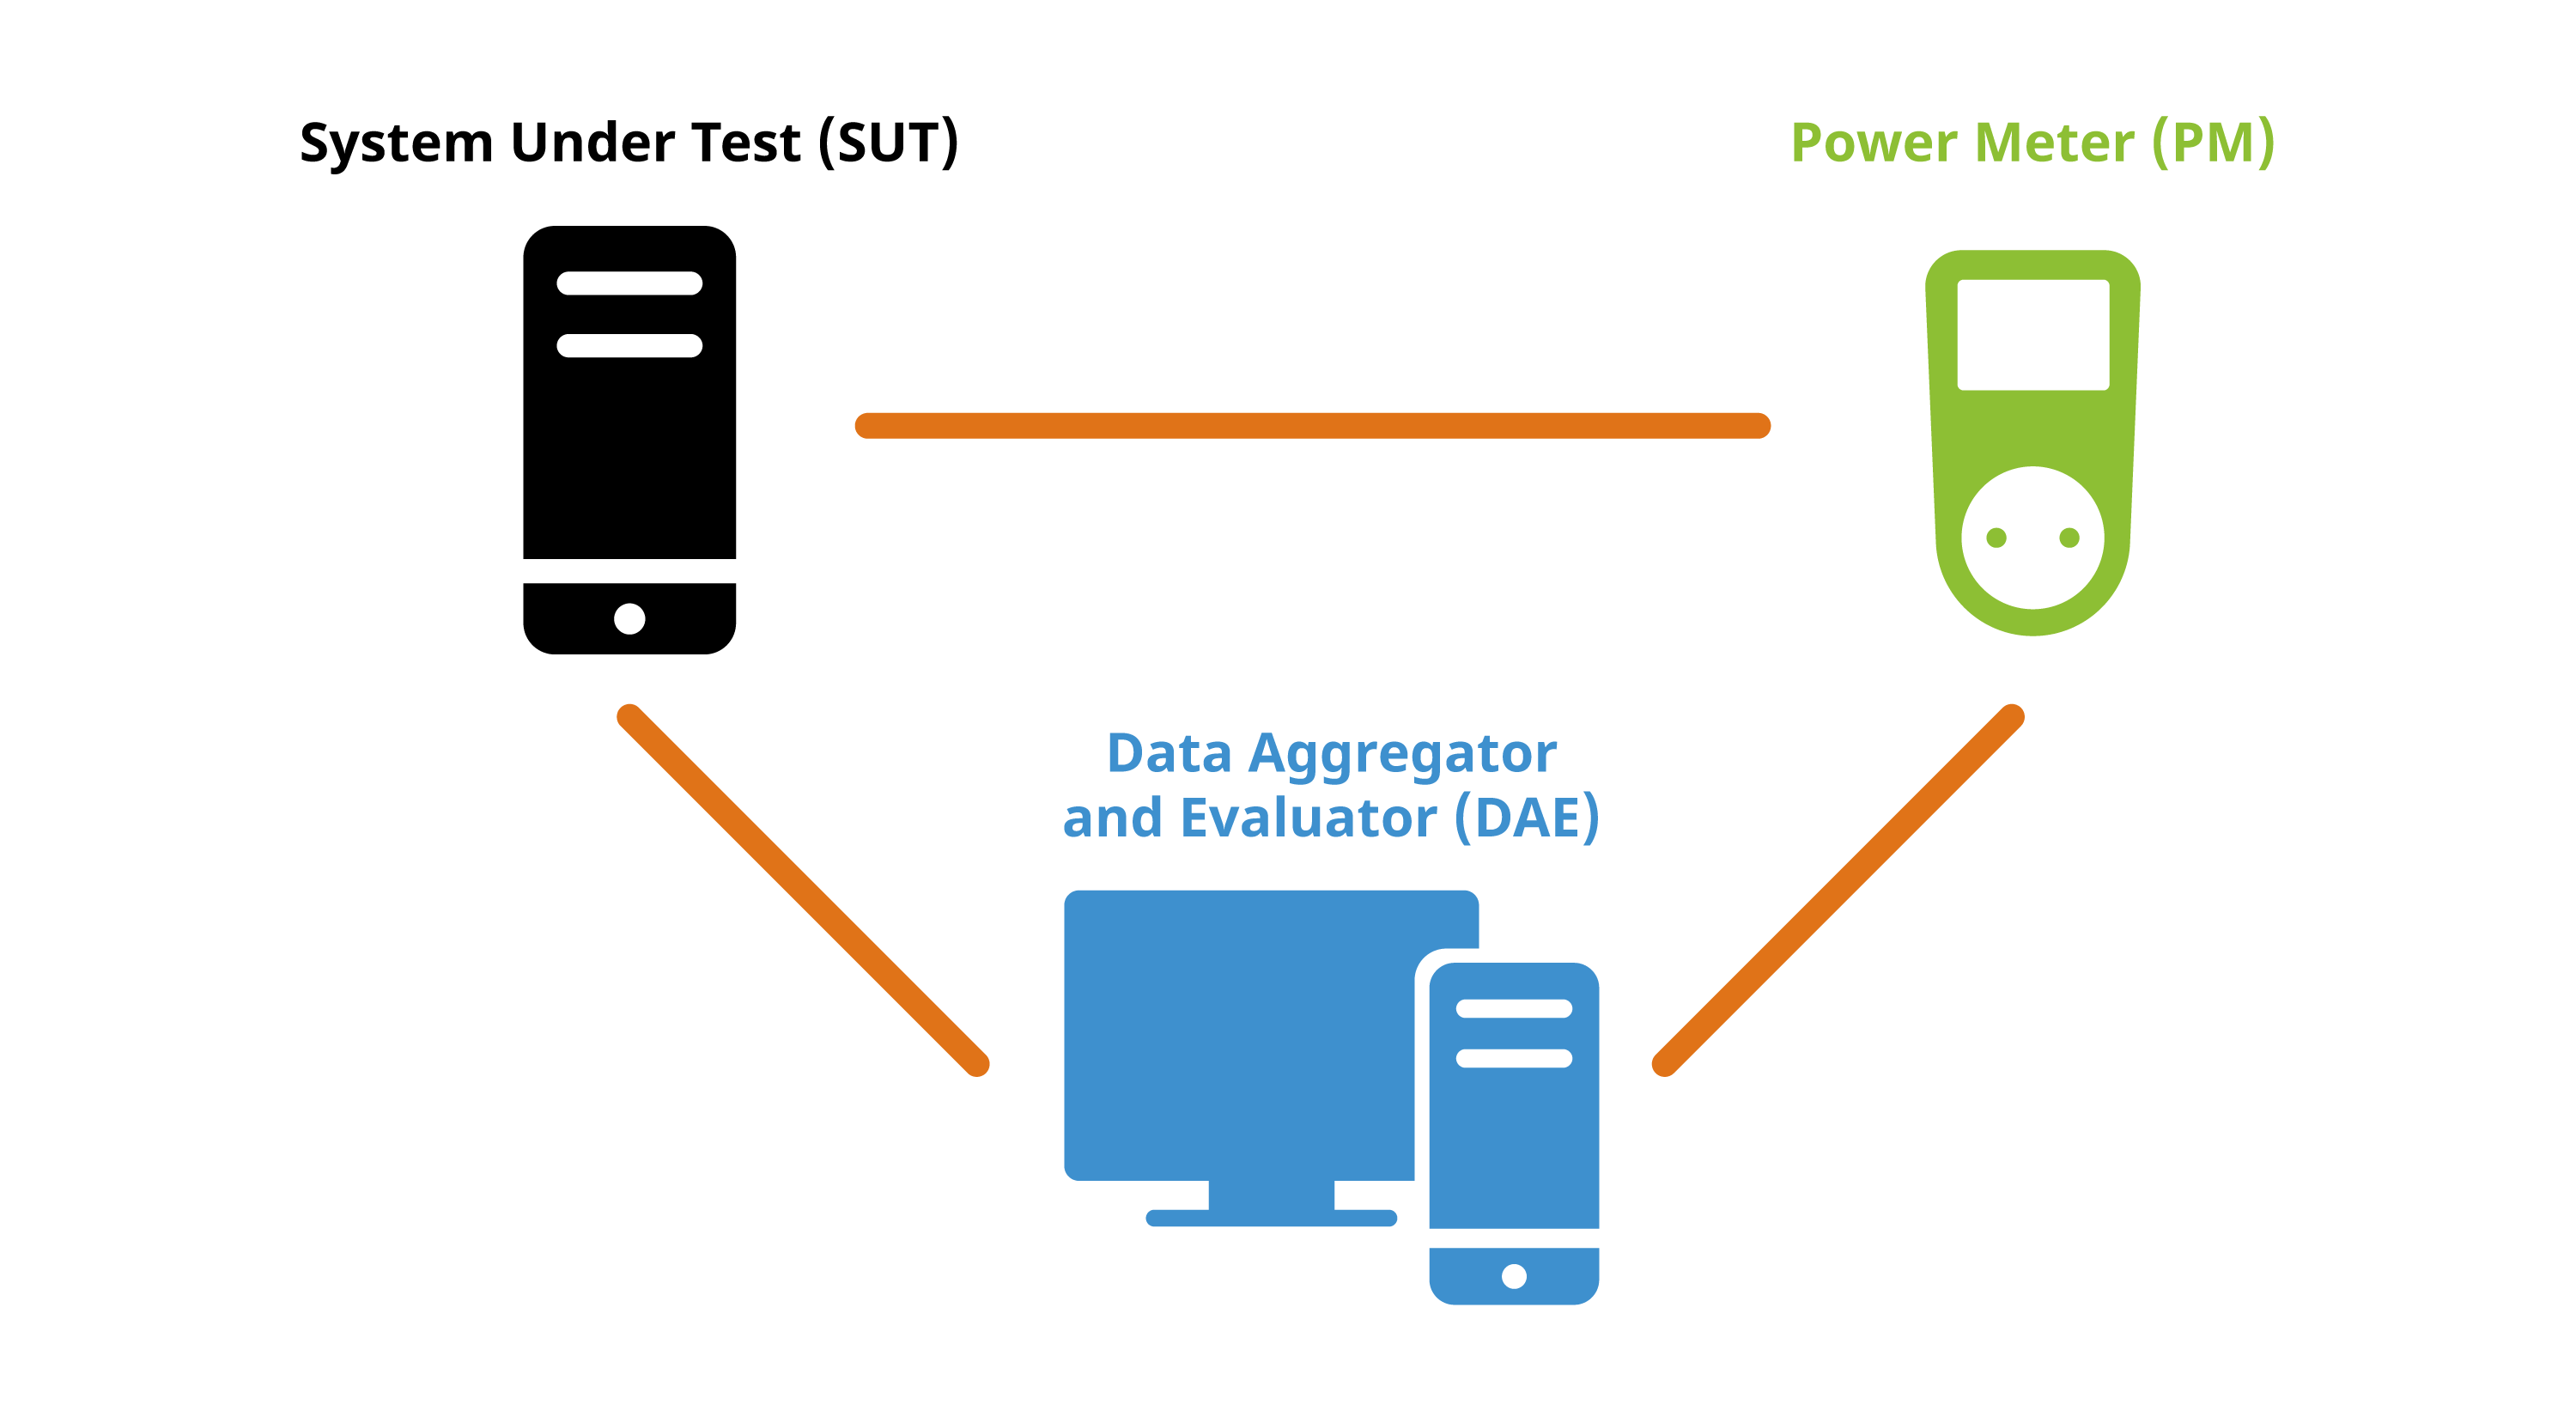
\includegraphics[width=10cm]{../img/sec3_lab-setup_modified.png}
    \end{figure}

    \subsection{Power meter}
    First, to measure the energy consumption of anything, a power meter is needed. This will be provided by the school and is of the brand Sirius. The device which is recommended by Blue Angel is the 'Gude Expert Power Control 1202 Series'. The power meter should at least do one measurement per second and also create additional system logs with timestamps. To create these logs, the recommended tool is 'Collectctl'. This tool logs system relevant data, like RAM usage, CPU loading, or network status (Blauer Engel, S. 36).
    The data, which is collected, has to be stored in CSV format. One of the benefits is, that KDE's 'LabPlot' can process the CSV data live to output the data. Still, the main reason for storing the data into CSV is, that the analysis tool OSCAR, which is provided by the Campus Birkenfeld, needs this format (KDE Eco Handbook).
    \subsection{Data Aggregator and Evaluator}
    The next part is a PC as Data Aggregator and Evaluator is needed, which collects and processes the data from the power meter. The recommended power meter of Blue Angel can be used with a Python script, to read out the measurement. The device used for this lab comes with it's own proprietary software. Using this would cross the ethical principles of KDE, as it is no free open source software and further is not available for Linux. Due to this the open source solution 'openDAQ' will be used, which can be used combined with C++ or Python.
    \subsection{System Under Test}
    Also a second PC is needed, which is the System Under Test(SUT) where the application will be executed on, and which delivers the measurement data in form of the power usage in the three test-case scenarios.
    Regarding the Computer System the requirement of Bluze Angel is, that the system has to be published to the market in the past few years, in other words it must not be published in the actual year. This ensures that the downward compatibility for running the software is given. This deviced will run the new Selenium scripts to perform the tests. Additionally 'Collectctl' will also be used to review side data (Blauer Engel, S. 41).
    Additionally to the basic software and hardware components, the SUT also has to be prepared a little bit. For making the tests, it has to be ensured, that any other energy consumption of the system is reduced to a minimum. In order to be able to provide that, the reccommodations of Blue Angel are as follows (KDE Eco Handbook):
    \begin{itemize}
        \item Format the harddrive of the device and install the operating system to make sure that only the OS is on the drive
        \item Shut off every process of the system, which is not needed for executing the scenarios
        \item Install the needed software
        \item Remove the cache between the tests, as it changes the original state of the system before each test
    \end{itemize}

    \section{Interfaces between used components}
    \section{Test the Lab-setup}